\documentclass[9pt]{article}
\usepackage[top=3cm, bottom=3cm, outer=3cm, inner=3cm]{geometry}
\usepackage{multicol}
\usepackage{graphicx}
\usepackage{url}
\usepackage{hyperref}
\usepackage{array}
\newcolumntype{x}[1]{>{\centering\arraybackslash\hspace{0pt}}p{#1}}
\usepackage{natbib}
\usepackage{multirow}
\usepackage[normalem]{ulem}
\useunder{\uline}{\ul}{}
\usepackage{listings}
\lstdefinestyle{ascii-tree}{
	literate={├}{|}1 {─}{--}1 {└}{+}1 
}
\lstset{basicstyle=\ttfamily,
	showstringspaces=false,
	commentstyle=\color{red},
	keywordstyle=\color{blue}
}
\usepackage{caption}
\usepackage{subcaption}
\usepackage{float}
\usepackage{array}
\usepackage{longtable}
\usepackage{tabularx}
\usepackage{adjustbox}
\usepackage[table]{xcolor}% http://ctan.org/pkg/xcolor
\usepackage{blindtext}
\renewcommand{\familydefault}{\sfdefault}
\usepackage{geometry}
\geometry{
	a4paper,
	total={190mm,257mm},
	left=10mm,
	top=20mm,
}
\newcolumntype{M}[1]{>{\centering\arraybackslash}m{#1}}
\newcolumntype{N}{@{}m{0pt}@{}}
%%%%%%%%%%%%%%%%%%%%%%%%%%%%%%%%%%%%%%%%%%%%%%%%%%%%%%%%%%%%%%%%%%%%%%%%%%%%
%%%%%%%%%%%%%%%%%%%%%%%%%%%%%%%%%%%%%%%%%%%%%%%%%%%%%%%%%%%%%%%%%%%%%%%%%%%%
\newcommand{\itemCourse}{Estructura de Datos y Algoritmos}
\newcommand{\itemUniversity}{Universidad Nacional de San Agustín de Arequipa}
\newcommand{\itemFaculty}{Facultad de Ingeniería de Producción y Servicios}
\newcommand{\itemDepartment}{Departamento Académico de Ingeniería de Sistemas e Informática}
\newcommand{\itemSchool}{Escuela Profesional de Ingeniería de Sistemas}
\newcommand{\itemPracticeNumber}{06}
\newcommand{\itemTheme}{Arbol AVL}
%%%%%%%%%%%%%%%%%%%%%%%%%%%%%%%%%%%%%%%%%%%%%%%%%%%%%%%%%%%%%%%%%%%%%%%%%%%%
%%%%%%%%%%%%%%%%%%%%%%%%%%%%%%%%%%%%%%%%%%%%%%%%%%%%%%%%%%%%%%%%%%%%%%%%%%%%
\usepackage[english,spanish]{babel}
\usepackage[utf8]{inputenc}
\AtBeginDocument{\selectlanguage{spanish}}
\renewcommand{\figurename}{Figura}
\renewcommand{\refname}{Referencias}
\renewcommand{\tablename}{Tabla} %esto no funciona cuando se usa babel
\AtBeginDocument{%
	\renewcommand\tablename{Tabla}
}
\usepackage{fancyhdr}
\pagestyle{fancy}
\fancyhf{}
\setlength{\headheight}{30pt}
\renewcommand{\headrulewidth}{1pt}
\renewcommand{\footrulewidth}{1pt}
\fancyhead[L]{\raisebox{-0.2\height}{
\includegraphics[width=3cm]{img/logo_episunsa.png}}}
\fancyhead[C]{\fontsize{7}{7}\selectfont	\itemUniversity \\ \itemFaculty \\ \itemDepartment \\ \itemSchool \\ \textbf{\itemCourse}}
\fancyhead[R]{\raisebox{-0.2\height}{
\includegraphics[width=1.2cm]{img/logo_abet}}}
\fancyfoot[C]{\itemCourse}
\fancyfoot[R]{Página \thepage}
\usepackage{listings}
\usepackage{color, colortbl}
\definecolor{dkgreen}{rgb}{0,0.6,0}
\definecolor{gray}{rgb}{0.5,0.5,0.5}
\definecolor{mauve}{rgb}{0.58,0,0.82}
\definecolor{codebackground}{rgb}{0.95, 0.95, 0.92}
\definecolor{tablebackground}{rgb}{0.8, 0, 0}
\lstset{frame=tb,
	language=bash,
	aboveskip=3mm,
	belowskip=3mm,
	showstringspaces=false,
	columns=flexible,
	basicstyle={\small\ttfamily},
	numbers=none,
	numberstyle=\tiny\color{gray},
	keywordstyle=\color{blue},
	commentstyle=\color{dkgreen},
	stringstyle=\color{mauve},
	breaklines=true,
	breakatwhitespace=true,
	tabsize=3,
	backgroundcolor= \color{codebackground},
}
\begin{document}
	
	\vspace*{10px}
	
	\begin{center}	
		\fontsize{17}{17} \textbf{ Informe de Laboratorio \itemPracticeNumber}
	\end{center}
	\centerline{\textbf{\Large Tema: \itemTheme}}
	%%%%%%%%%%%%%%%%%%%%%%%%%%%%%%%%%%%%%%%%%%%%%%%%%%%%%%%%%%%%%%%%%%%%%%%%%%%%
	\begin{adjustbox}{width=\textwidth}
		\begin{tabularx}{\textwidth} {
				| >{\raggedright\arraybackslash}X 
				| >{\raggedright\arraybackslash}X 
				| >{\raggedright\arraybackslash}X 
				| >{\raggedright\arraybackslash}X
				| >{\raggedright\arraybackslash}X
				| >{\raggedright\arraybackslash}X |}
			\hline
			\rowcolor{tablebackground}
			\multicolumn{6}{ | c | }{\color{white}\textbf{INFORMACIÓN BÁSICA}} \\
			\hline
			\textbf{ASIGNATURA:}& \multicolumn{5}{ | l | }{\textbf{\itemCourse}} \\
			\hline
			\textbf{TÍTULO DEL TRABAJO:} & \multicolumn{5}{ | l | }{Trabajo Final: Detector de plagio} \\
			\hline
			\textbf{NÚMERO DE TRABAJO:}& 07 & \textbf{AÑO LECTIVO:} & 2023-A & \textbf{NRO. SEMESTRE:} & III \\
			\hline
			\textbf{FECHA DE PRESENTACIÓN:} & 08/08/23 &\textbf{HORA DE PRESENTACIÓN:}& \multicolumn{3}{ | l | }{23:59} \\
			\hline
			\multicolumn{4}{ | l | }{\textbf{INTEGRANTE (s)}} & \textbf{NOTA (0-20)} & \\
			\hline
			\multicolumn{6}{ | l | }{\textbf{Hidalgo Chinchay, Paulo Andre}}\\
			\multicolumn{6}{ | l | }{\textbf{Betanzos Rosas, Taylor Anthony}}\\
			\multicolumn{6}{ | l | }{\textbf{Villafuerte Ccapira Frank Alexis}} \\
			\hline
			\multicolumn{6}{ | l | }{\textbf{DOCENTE(s):}} \\
			\multicolumn{6}{ | l | }{Mg. Edith Giovanna Cano Mamani} \\
			\hline
		\end{tabularx}
	\end{adjustbox}
	
	%%%%%%%%%%%%%%%%%%%%%%%%
	\begin{longtable}{|p{15cm}|}
		\caption{Mi tabla extendida}\\
		\hline 
		\rowcolor{tablebackground}
		\color{white}\textbf{INTRODUCCIÓN}  \\
		\hline 
		 En el campo de la investigación el robo de  propiedad intelectual es un problema muy grande, y la preocupación ante este problema crece aún más debido a la facilidad que nos ofrece la tecnología para acceder a la información.\\
		 En el presente trabajo presentaremos la implementación de un detector de plagio textual, el cual buscará aspectos similares entre un párrafo base y varios documentos; y a partir de esto dará un veredicto.\\
		\hline 
		%%%%%%%%%%%%
		\rowcolor{tablebackground}
		\color{white}\textbf{MARCO CONCEPTUAL}  \\
		\hline 
		\textbf{TRIE}  \\
		Un trie es una estructura de datos de tipo árbol que permite
		la recuperación de información.
		La información almacenada en un trie es un conjunto de claves, donde 
		una clave es una secuencia de símbolos pertenecientes a un alfabeto. 
		Las claves son almacenadas en las hojas del árbol y los nodos internos 
		son pasarelas para guiar la búsqueda. El árbol se estructura de forma 
		que cada letra de la clave se sitúa en un nodo de forma que los hijos
		de un nodo representan las distintas posibilidades de símbolos diferentes
		que pueden continuar al símbolo representado por el nodo padre. Por tanto 
		la búsqueda en un trie se hace de forma similar a como se hacen las búsquedas 
		en un diccionario[1]\\	
		
		\textbf{PLAGIO}  \\
		Según la RAE, el plagio es la acción de plagiar, el cual consiste copiar obras ajenas y darlas como propias[2,3]\\	
		 
		\textbf{DETECTOR DE PLAGIO}  \\
		Es el proceso de detectar las similitudes de contenido, el cual se realizaba mediante la detección humana. Gracias a la llegada de la tecnología, este proceso  facilitó la tarea, que normalmente llevaba una gran cantidad de tiempo[4].\\	
		\hline 
		%%%%%%%%%%%%
		\rowcolor{tablebackground}
		\color{white}\textbf{SOLUCIONES Y PRUEBAS}  \\
		\hline
		El detector de plagio requiere una comparación entre palabras del texto de referencia y el texto evaluado, por lo cual debemos almacenar las palabras del primer texto de tal manera que podamos encontrarlos con facilidad.\\
		En este caso creamos un Trie, el cual es un árbol que almacenará las palabras. En nuestro código, cada Nodo del Trie tendrá un arreglo de 27 posiciones, representando a cada una de las letras del alfabeto. Según la letra que se vaya a almacenar se agrega un nodo hijo a la posicion correspondiente.\\
		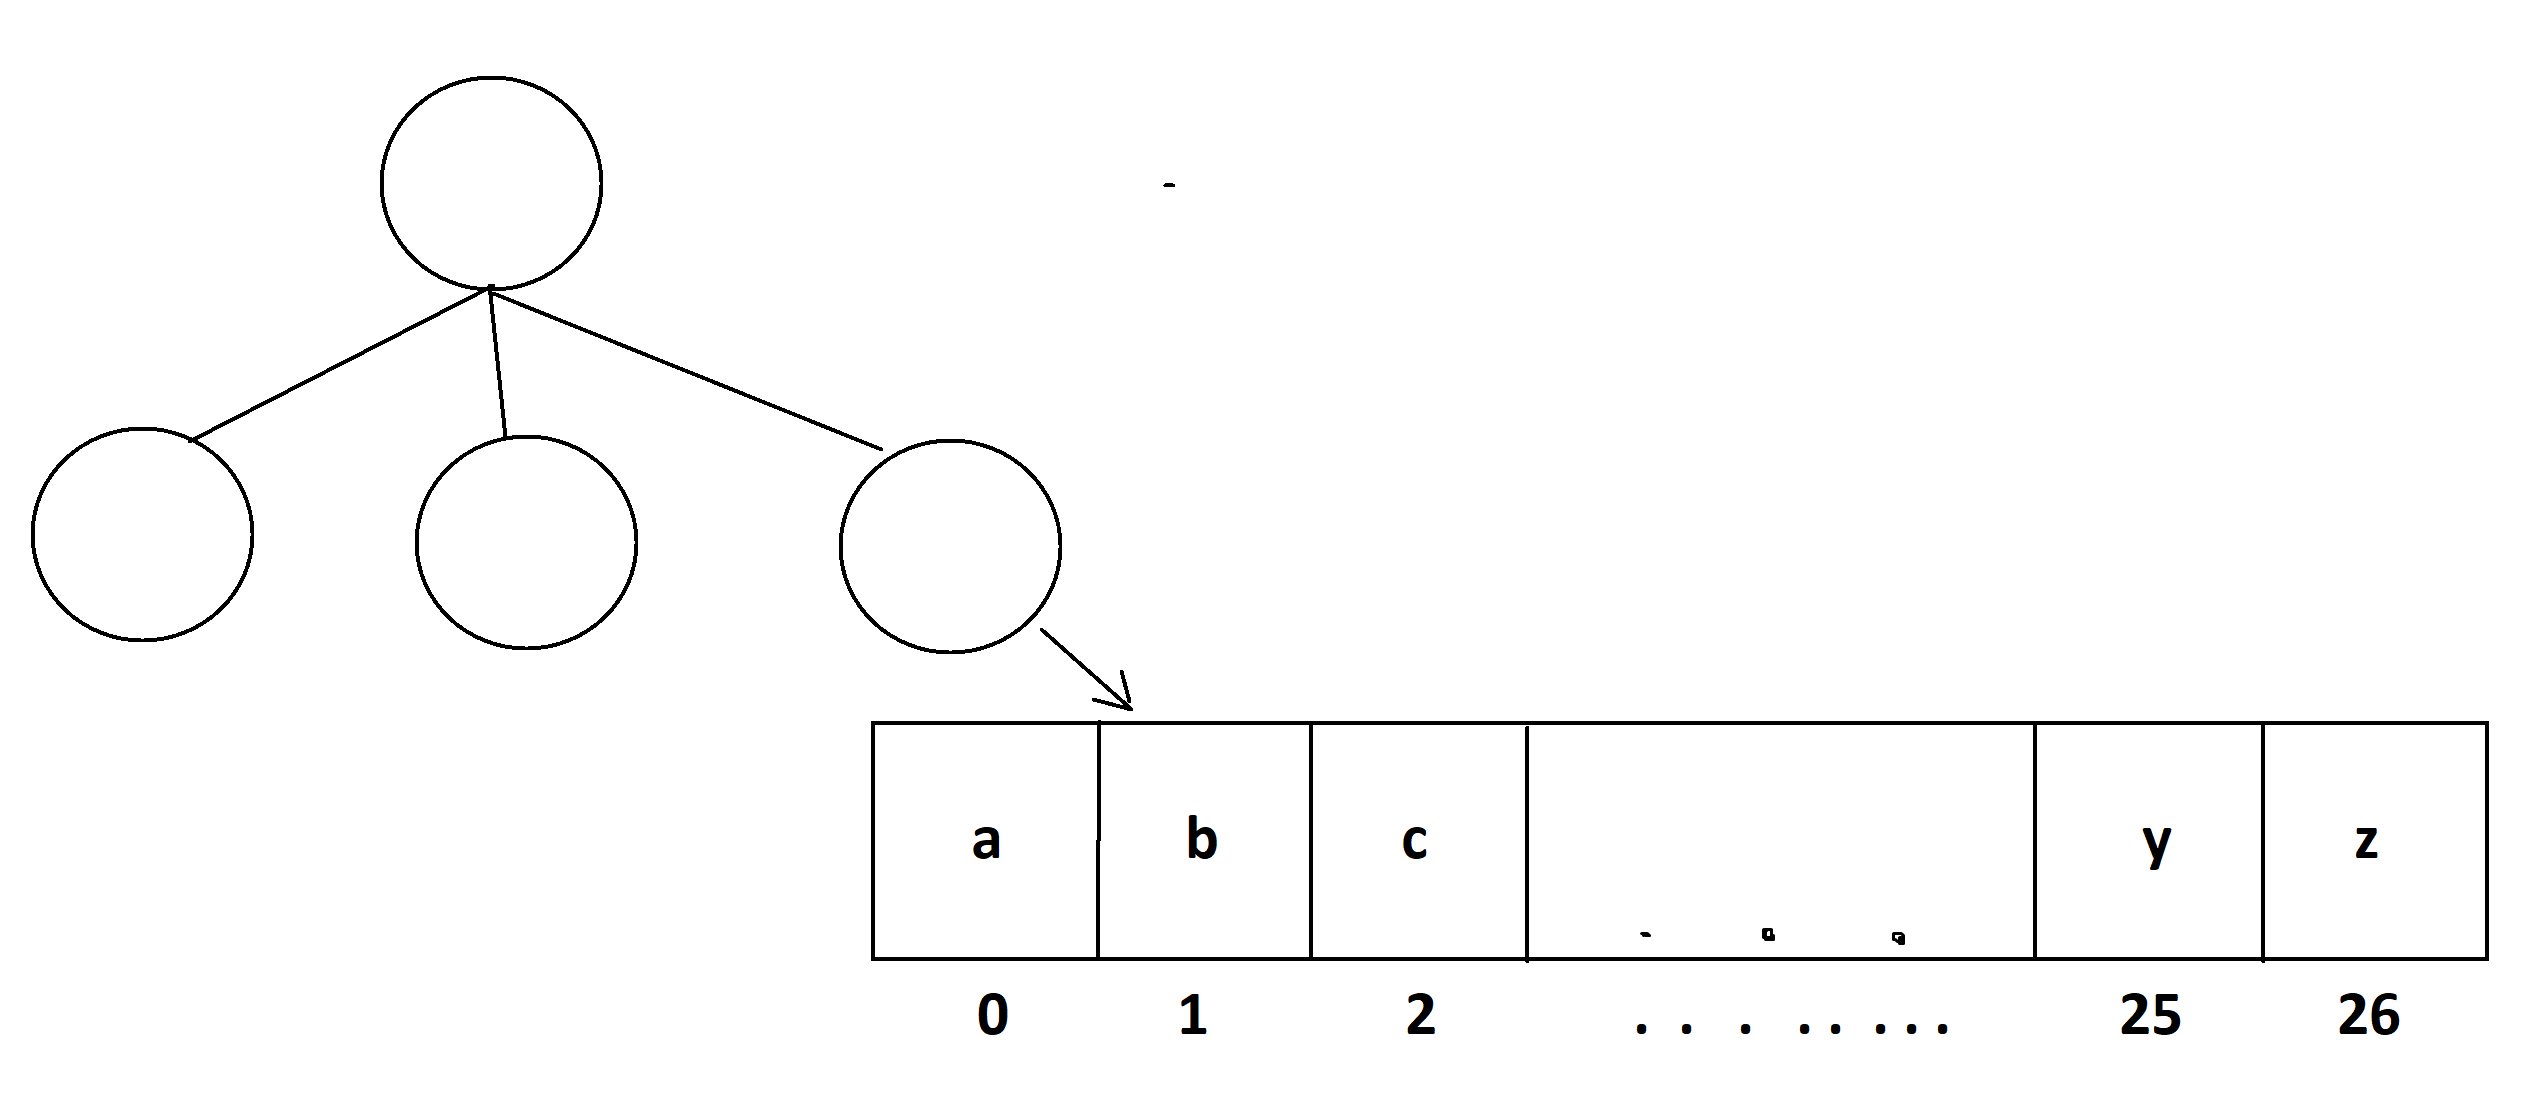
\includegraphics[width=14cm]{img/trie.png}\\
		Para corresponder la posicion de las letras debemos asignar un valor numérico teniendo a la letra a como 0, b como 1 y así sucesivamente. \\
		Para lograr esto usaremos el código ascii de cada letra, y le restaremos el valor de la "a", así obtendremos un valor relativo a las posiciones del alfabeto.\\
		
		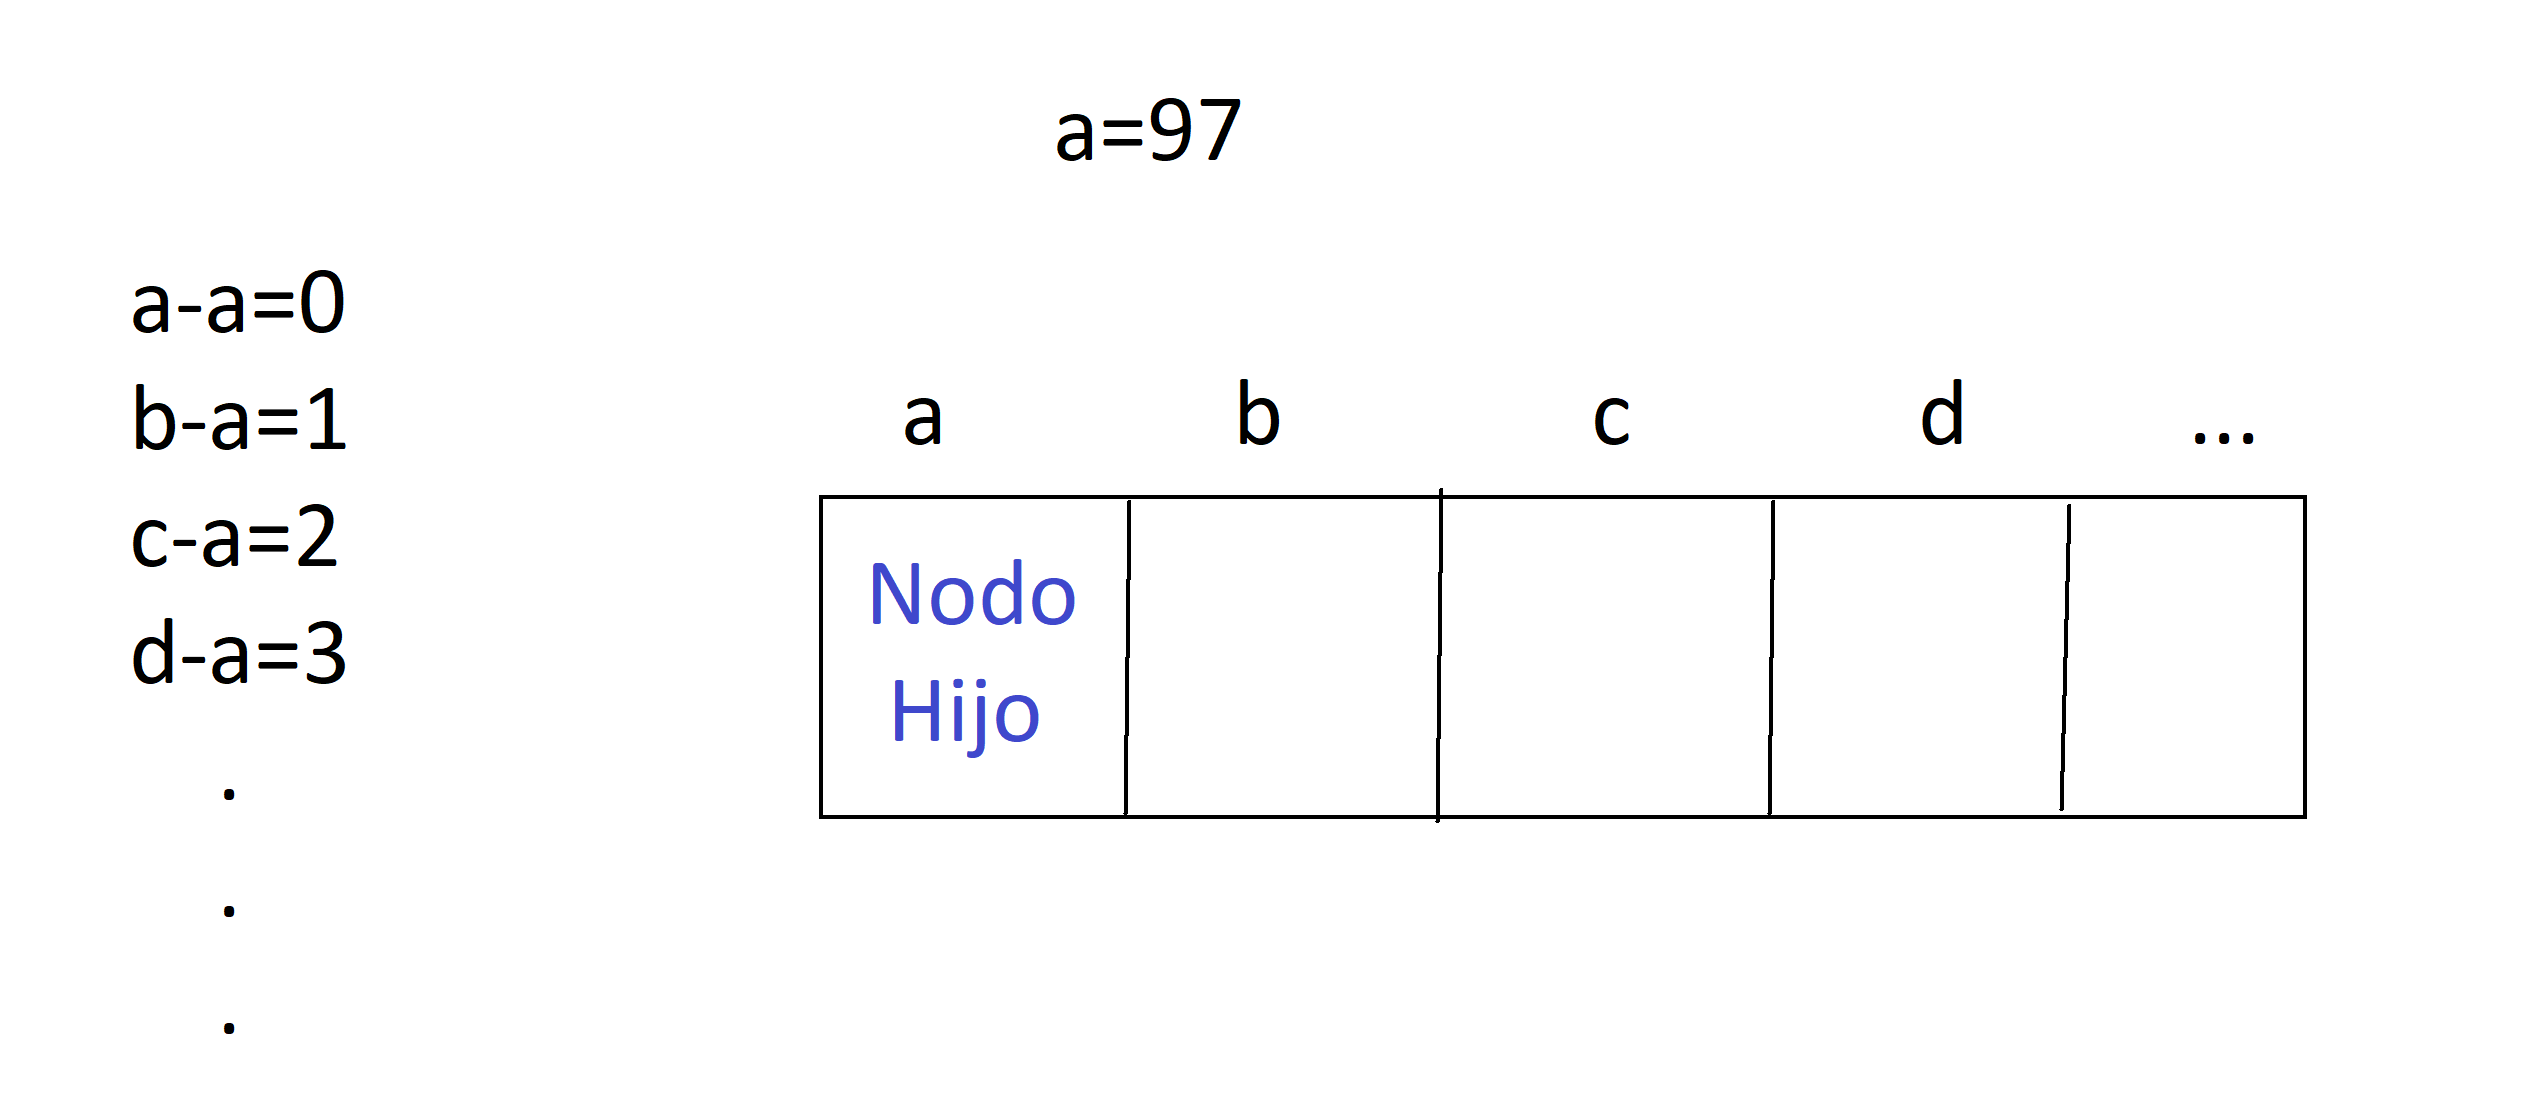
\includegraphics[width=14cm]{img/asignacionLetras.png}\\
		El procedimiento de detección de plagio requiere que tengamos un documento de referencia.\\
		Usaremos la clase PlagiarismChecker para obtener el contenido de los documentos y agregar las palabras al Trie que será almacenado dentro de esta misma clase.\\
		Mediante el botón de añadir archivo de la interfaz obtendremos el texto que contiene y agregaremos todas sus palabras al trie.\\
		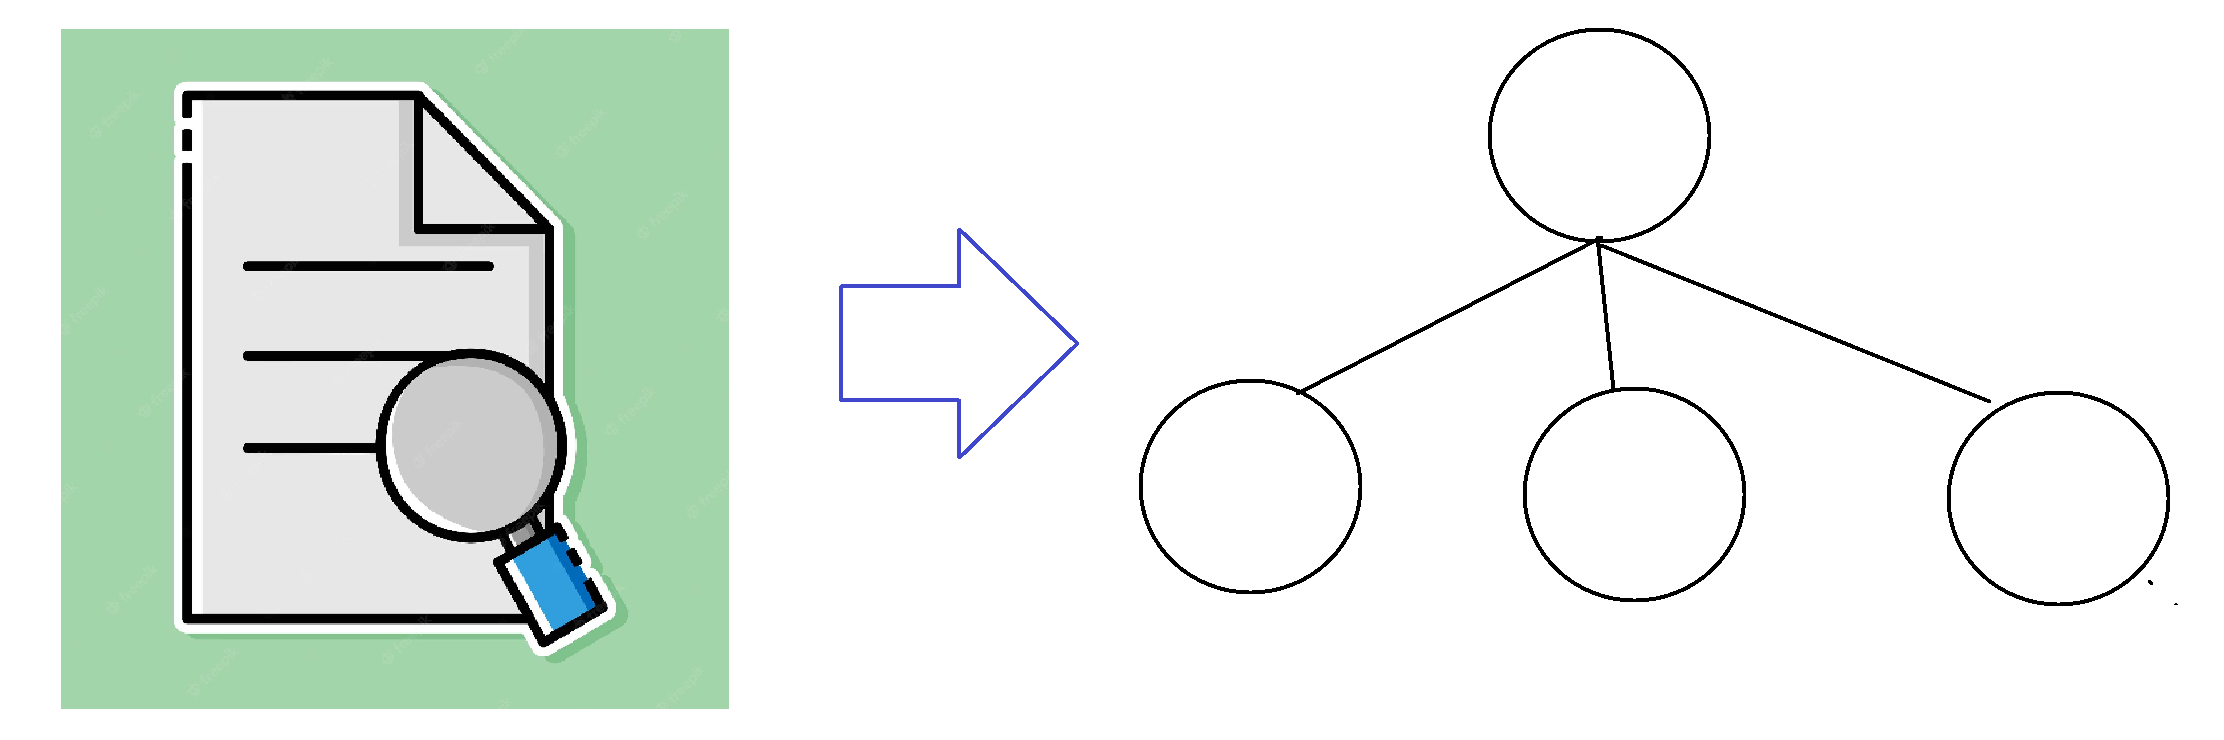
\includegraphics[width=14cm]{img/importarTexto.png}\\
		La métrica utilizada para el veredicto es el porcentaje de palabras similares del texto de referencia en relación a todas las palabras existentes en dicho texto.
		La clase ResulChacker buscará cada palabra en el trie e irá contando los resultados similares, luego lo comparará con la cantidad de palabras totales multiplicado por 0,2.
		Por tanto si el número de similitudes supera el 20\% el sistema alertará sobre plagio.
		Se compara cada uno de los documentos ingresados y la clase retornará un arreglo de booleanos que servirán a la interfaz para enviar un aviso de los resultados por cada documento.\\
		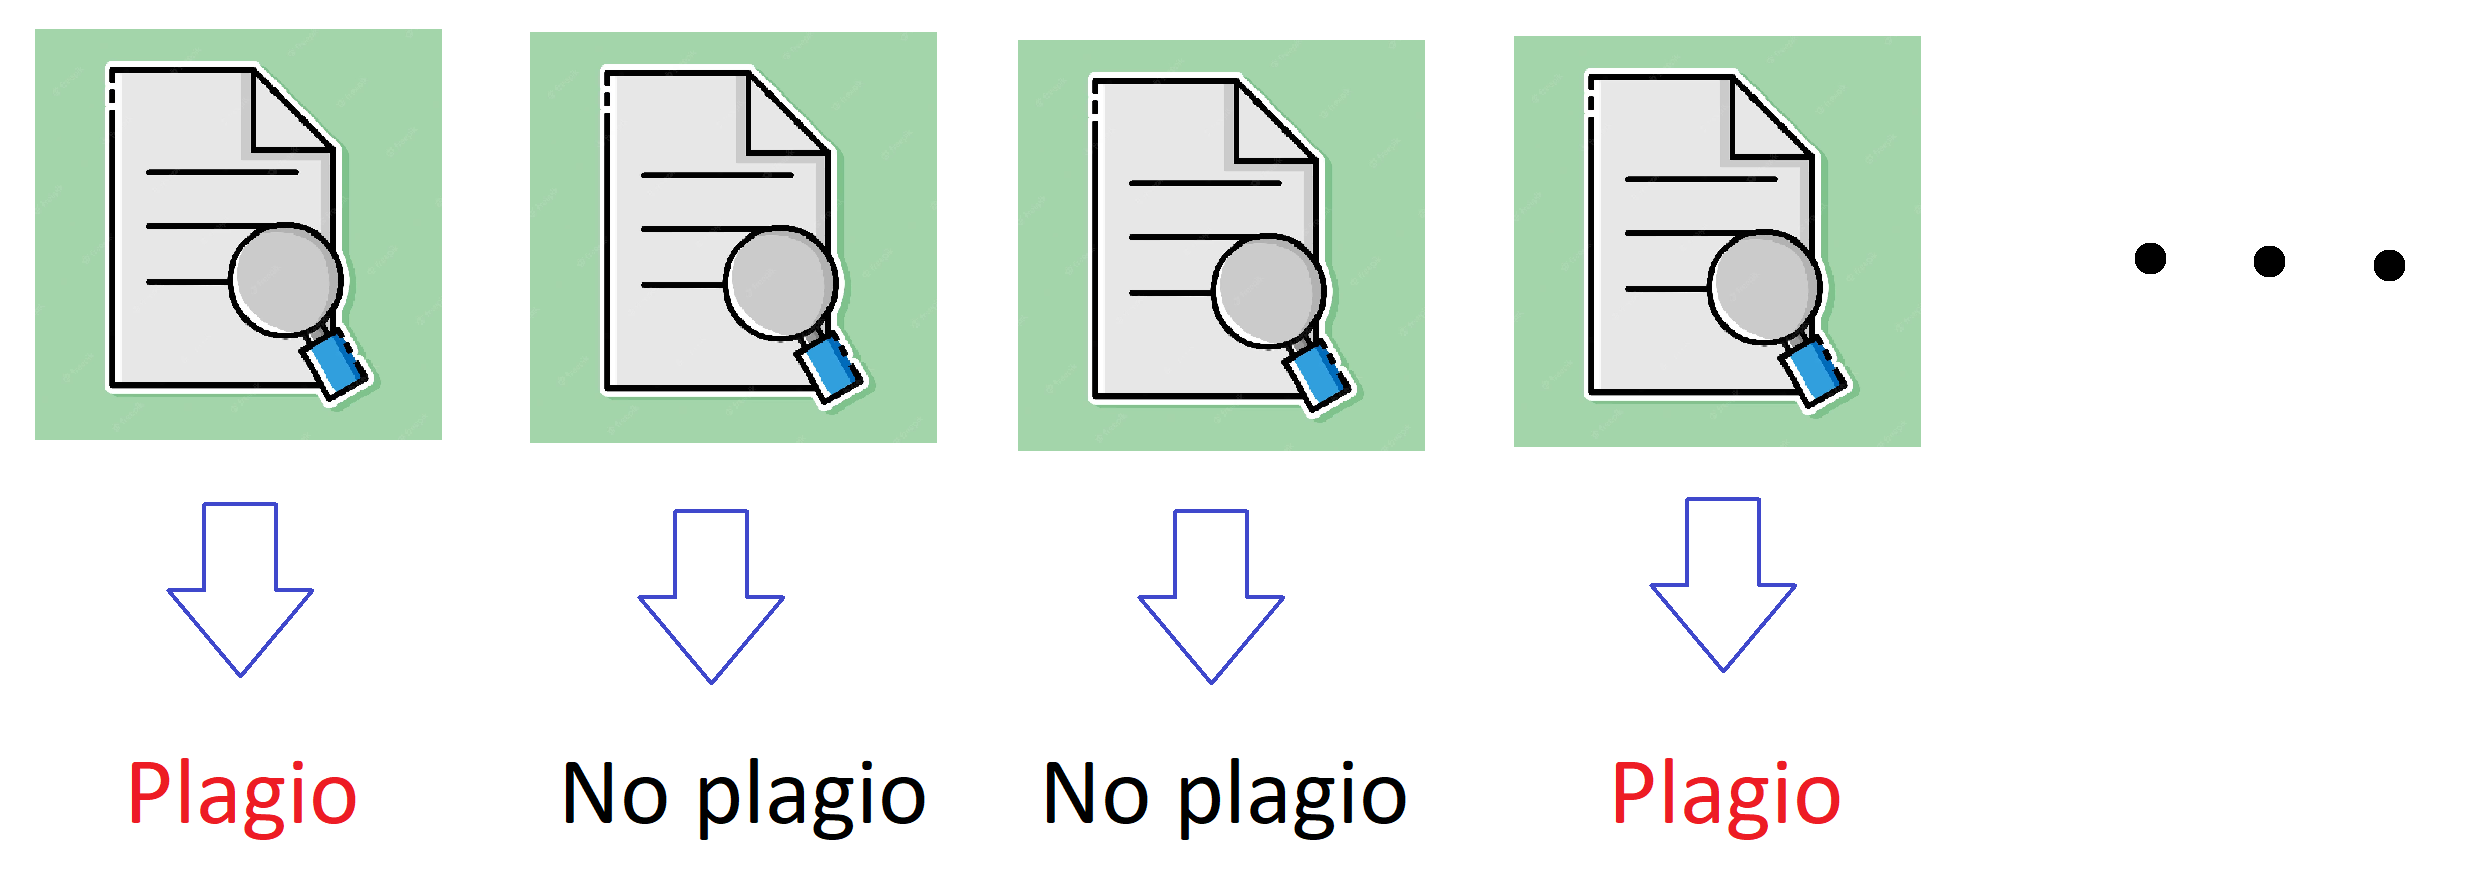
\includegraphics[width=14cm]{img/resultadosMultiples.png}\\
		
		En este caso usamos la clase ResulChacker dentro de PlagiarismChecker para poder enviarle el trie como parámetro.\\
	
		\hline
		%%%%%%%%%%%%			
	\end{longtable}
	%%%%%%%%%%%%%%%%%%%%%%%%
	\begin{table}[H]
		\begin{tabular}{|p{15cm}|}
			\hline 
			\rowcolor{tablebackground}
			\color{white}\textbf{LECCIONES APRENDIDAS Y CONCLUSIONES}  \\
			\hline 
			Durante el proceso de ejecución de este proyecto aprendimos a utilizar los árboles TRIE para facilitar la búsqueda de palabras específicas y verificar su existencia en un texto.\\
			Ademas aprendimos, a grandes rasgos, como funciona un detector de plagio textual y cómo el usar TRIES facilita el proceso de comparación y determinar que tan similar es el documento de referencia con el párrafo evaluado.\\
		\hline 
		%%%%%%%%%%%%
		\rowcolor{tablebackground}
		\color{white}\textbf{REFERENCIAS Y BIBLIOGRAFÍA}  \\
		\hline 
		\textbf{[1]\url{https://es.wikipedia.org/wiki/Trie}}\\
		\textbf{[2]\url{https://dle.rae.es/plagio}}\\
		\textbf{[3]}\url{https://dle.rae.es/plagiar#CU0knYP}\\
		\textbf{[4]}\url{	https://www.ayudauniversitaria.com/detector-de-plagio/}\\
	
	
		\hline 
		%%%%%%%%%%%%			
	\end{tabular}
\end{table}
%%%%%%%%%%%%%%%%%%%%%%%%
\end{document}
